%\makeatletter
%\def\toclevel@chapter{-1}
%\makeatother

\chapter{Conclusion et perspectives}
%\addtocontents{toc}{\bigskip}
%\addcontentsline{toc}{chapter}{Conclusion et perspectives}

Dans ce manuscrit, nous avons rapporté la mesure expérimentale du temps de diffusion élastique faisant suite aux travaux de Jérémie Richard \citep{richard2015propagation}, dont nous avons étudié le comportement sur une large gamme de paramètres, sondant les régimes de diffusion faible et de diffusion forte. En complétant notre étude basée sur des potentiels \speckle\ par la simulation d'un potentiel gaussien, nous avons pu examiner quantitativement la pertinence du critère $k_{\mathrm{i}}\ls\sim 1$ de validité de l'approximation de Born. Nous avons ainsi montré la une forte influence de la distribution du potentiel sur la position de la transition entre les régimes de diffusion faible et de diffusion forte. 

%Dans le but d'étendre le domaine de validité de l'approximation de Born, nous avons calculé le second ordre du développement de Born de la \selfenergy , permettant de décrire le comportement asymétrique du temps de diffusion élastique dans un régime de désordre et d'impulsion faibles. L'approximation auto-consistante de Born fournit une estimation tout à fait convaincante du temps de diffusion élastique pour un désordre gaussien, cependant elle échoue à décrire le cas des désordres de type \speckle . En comparant le temps de diffusion élastique au temps caractéristique extrait des fonctions spectrales mesurées $A(\mathbf{k}=0,E=\hb\delta)$, nous avons montré que la connaissance fine des détails de la fonction spectrale est capitale pour décrire correctement la dynamique du système. 

Dans le but de décrire le comportement du temps de diffusion élastique dans le régime de désordre fort, nous avons utilisé le formalisme des fonctions spectrales pour estimer un temps de vie caractéristique $\taus^{\mathrm{sf}}$. En comparant le temps de diffusion élastique au temps caractéristique extrait des fonctions spectrales mesurées $A(\mathbf{k}=0,E=\hb\delta)$, nous avons montré que la connaissance fine des détails de la fonction spectrale est capitale pour décrire correctement la dynamique du système. L'excellent accord entre nos différentes données expérimentales illustre donc la cohérence de nos deux approches, temporelle et dans le domaine des énergies.

Ces études ont montré le cruel besoin de prédictions quantitatives de la fonction spectrale pour la compréhension de phénomènes de transport plus complexes, tels que la localisation d'Anderson. Plus particulièrement, les désaccords observés entre les différentes expériences, les simulations et les théories s'attachant à décrire la transition de phase d'Anderson à trois dimensions trouvent leur origine dans la difficulté à déterminer expérimentalement et numériquement la distribution d'énergie de l'onde dans le désordre \citep{pasek2017anderson}.









\section{Vers l'étude du régime critique}
%Une difficulté rencontrée par les trois expériences présentées dans la section \ref{sc:etat_art_transition} correspond à l'élargissement de la distribution d'énergie des atomes dans le désordre, qui peut s'interpréter comme une résolution en énergie $\Delta E$. Notamment, le couplage réalisé entre les atomes et le désordre implique que cette résolution en énergie est au moins aussi grande que le seuil de mobilité $\Delta E \geq \Ec$. La détermination du seuil de mobilité requiert alors une connaissance précise de la fonction spectrale $A(\mathbf{k},E)$. De plus, l'étude des exposants critiques s'avère impossible en raison du manque de maîtrise du paramètre de contrôle (l'énergie des atomes) autour de la transition. 

%L'approche spectroscopique radio-fréquence développée par l'équipe permet d'adresser ces deux limitations. Celle-ci ayant mené à la mesure de la fonction spectrale $A(\mathbf{k}=0,E)$ pour des désordres de type \speckle\ attractif et répulsif, l'équipe a ainsi mis en évidence le comportement pathologique du \speckle\ répulsif utilisé dans les expériences pionnières de la localisation d'Anderson à trois dimensions. De plus, la résolution en énergie obtenue n'est plus limitée que par le temps de couplage de la spectroscopie $\Delta E \sim h/t_0$. Il apparaît donc possible de réaliser une expérience pour laquelle $\Delta E \ll \Ec$, et qui permettrait de sonder le régime critique. De plus, cette approche permet d'étendre l'étude du régime critique à des désordres attractifs, pour lesquels le comportement du seuil de mobilité n'est pas aussi régulier que pour les désordre répulsifs exclusivement utilisés jusqu'à présent \citep{delande2014mobility}.

\begin{figure}
\centering
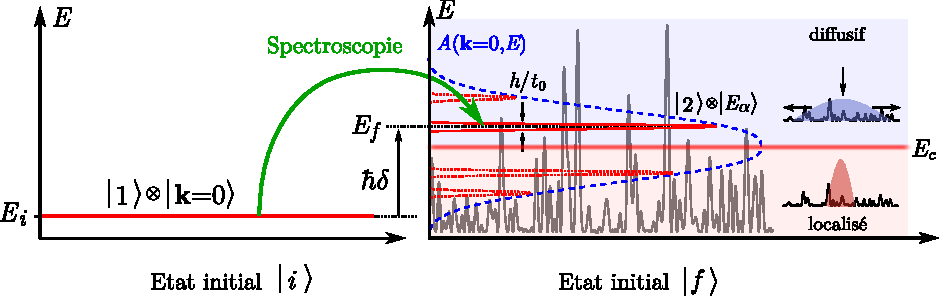
\includegraphics[width=\textwidth]{Fig/Conclusion/spectro_transition_anderson.pdf}
\caption{\textbf{Étude spectroscopique de la transition d'Anderson.} Une approcche spectroscopique de la transition d'Anderson se décomposerait selon deux étapes. Une première étape de chargement du désordre consisterait à transférer une partie du nuage à une énergie $\hb\delta$ dans le désordre à l'aide d'un couplage radio-fréquence. La résolution en énergie alors obtenue serait limitée par le temps de couplage $t_0$, donnant $\Delta E \sim h/t_0$. La seconde étape permettrait de caractériser l'énergie adressée en terme de localisation ou de diffusion en procédant à l'expansion de la partie transférée du nuage.}
\label{fig:spectro_transition_anderson}
\end{figure}

L'étude spectroscopique du régime critique de la transition d'Anderson apparaît naturellement comme prochaine étape expérimentale de l'équipe. En effet, on peut aisément imaginer le protocole de mesure du régime critique comme une extension de la spectroscopie radio-fréquence représentée figure \ref{fig:spectro_transition_anderson}:
\begin{itemize}
\item[\textendash] Une première étape consiste à charger le désordre dans un état d'énergie bien définie à l'aide d'un transfert spectroscopique. Les atomes sont ainsi transférés dans le désordre à une énergie $\hb\delta$ fixée par le désaccord de la transition de à deux-photons, avec une résolution d'énergie $\Delta E$ limitée par le temps de couplage.
\item[\textendash] Une seconde étape d'expansion de la partie transférée du nuage. En suivant l'évolution temporelle du nuage dans le désordre, il est possible de caractériser l'énergie $\hb\delta$ adressée en terme de localisation ou de diffusion à l'aide d'un arrêt de l'expansion ou de saturation de la densité centrale \citep{billy2008direct, jendrzejewski2012three}.
\end{itemize}

Cette mesure du régime critique n'a pas pu être réalisée lors de la mesure des fonctions spectrales en raison de deux limitations expérimentales. Une première limitation provient du temps de vie très limité des atomes en présence de désordre en raison du faible désaccord nécessaire à l'approche de désordre dépendant de l'état interne. Le temps de vie ainsi obtenu est de plusieurs ordres de grandeur inférieur aux temps nécessaires pour pouvoir qualifier un état comme localisé. Une nouvelle approche de désordre bichromatique détaillée au chapitre \ref{ch:Speckle} devrait ainsi dépasser cette limitation en permettant de s'éloigner de la résonance atomique tout en conservant le caractère sélectif en état de spin. 

%Une seconde limitation provient de l'utilisation du champ magnétique \emph{magique} à $\Bzero^*\approx\SI{3.2}{\gauss}$ qui permet de s'affranchir des fluctuations de champ magnétique lors du transfert spectroscopique. L'utilisation d'un tel bas champ génère un piégeage de fréquence $\omega/2\pi\sim\SI{5}{\hertz}$, empêchant de procéder à des expansions dans le désordre pour des durées de l'ordre de la seconde. L'étude de la lévitation magnétique présentée au chapitre \ref{ch:new_exp} montre que décomprimer ce piégeage magnétique en augmentant le biais $\Bzero$ s'accompagne d'un déplacement du nuage, qu'il convient de compenser afin de conserver la résolution d'énergie obtenue par spectroscopie. 
Une seconde limitation provient de l'utilisation du bas champ magnétique \emph{magique} $\Bzero^*$, empêchant de procéder à des expansions dans le désordre pour des durées de l'ordre de la seconde. La calibration fine du potentiel magnétique présentée au chapitre \ref{ch:new_exp} nous permettra de décomprimer le piégeage magnétique tout en conservant la résolution d'énergie obtenue par spectroscopie. 

Ces deux limitations ont ainsi fait l'objet d'investigations expérimentales poussées suite à nos travaux autour de la chambre de science au cours de ma thèse. Ceux-ci ont d'ailleurs permis d'obtenir de meilleurs condensats grâce à l'amélioration de notre évaporation optique, ainsi qu'un meilleur contrôle des champs magnétiques. Suite à ces travaux, l'équipe a récemment pu obtenir une résolution en énergie de $\Delta E/h\sim\SI{5}{\hertz}$ pour une durée de transfert de $t_0=\SI{200}{\milli\second}$, améliorée d'un facteur 2 par rapport à la résolution obtenue lors de la mesure des fonctions spectrales tout en restant limitée par transformée de Fourier.







\section{Signatures de la localisation d'Anderson dans l'espace des impulsions}
Comme nous avons pu voir dans le chapitre \ref{ch:TauS_PRL}, l'évolution temporelle de la fonction d'onde dans l'espace des impulsions révèle de nombreuses quantités microscopiques de la propagation d'onde en milieu désordonné, telles que le temps de diffusion élastique \citep{richard2019elastic}, le temps de transport donné par l'isotropisation de la distribution de vitesses \citep{plisson2013momentum}, mais aussi des signatures d'effets de localisation \citep{cherroret2012coherent}.

\subsection{Rétro-diffusion cohérente}
Le pic de rétro-diffusion cohérente (\emph{CBS} pour l'anglais \emph{Coherent BackScattering}) est une signature d'effets de localisation faible dans l'espace des vitesses. Celui-ci résulte d'interférences constructives dans la direction $\etat{\mathbf{k}_{\mathrm{f}}=-\mathbf{k}_{\mathrm{i}}}$ entre chemins de diffusions symétriques par renversement du temps lorsqu'une onde plane initiale $\etat{\mathbf{k}_{\mathrm{i}}}$ est plongée dans un milieu désordonné (voire figure \ref{fig:cbs_cfs}$\mathrm{a_1}$). Le CBS a pu être observé à l'aide d'un protocole similaire à celui utilisé pour étudier le temps de diffusion élastique \citep{jendrzejewski2012coherent} sous la forme d'un pic émergeant de l'anneau de diffusion élastique dans la direction $\mathbf{k}_{\mathrm{f}}=-\mathbf{k}_{\mathrm{i}}$ (voir figure \ref{fig:cbs_cfs}$\mathrm{a_2}$), et la manipulation de la symétrie par renversement du temps a mis en évidence le caractère cohérent de celui-ci \citep{muller2015suppression}.

Dans de récents travaux, l'équipe de Dominique Delande a montré que l'évolution temporelle de la largeur du pic CBS pouvait être une signature de la localisation d'Anderson \citep{ghosh2015coherent}. En particulier, ils ont montré que 
\begin{equation}
k_{\mathrm{i}} \Delta\theta_{\mathrm{CBS}}(t) \sim \left\lbrace \begin{aligned}
& 1/\sqrt{D(E)t}  \quad &&\text{pour } E>\Ec \text{ ,}\\
& 1/t^{1/3} \quad &&\text{pour } E=\Ec \text{ ,}\\
& 1/\xi(E) \quad &&\text{pour } E<\Ec \text{ ,}
\end{aligned}\right.
\label{eq:largeur_cbs}
\end{equation}
que l'on peut aisément interpréter à l'aide de l'évolution temporelle de la taille du paquet d'onde dans l'espace réel $\Delta x\sim (k_{\mathrm{i}} \Delta \theta_{\mathrm{CBS}})^{-1}$.

\begin{figure}
\centering
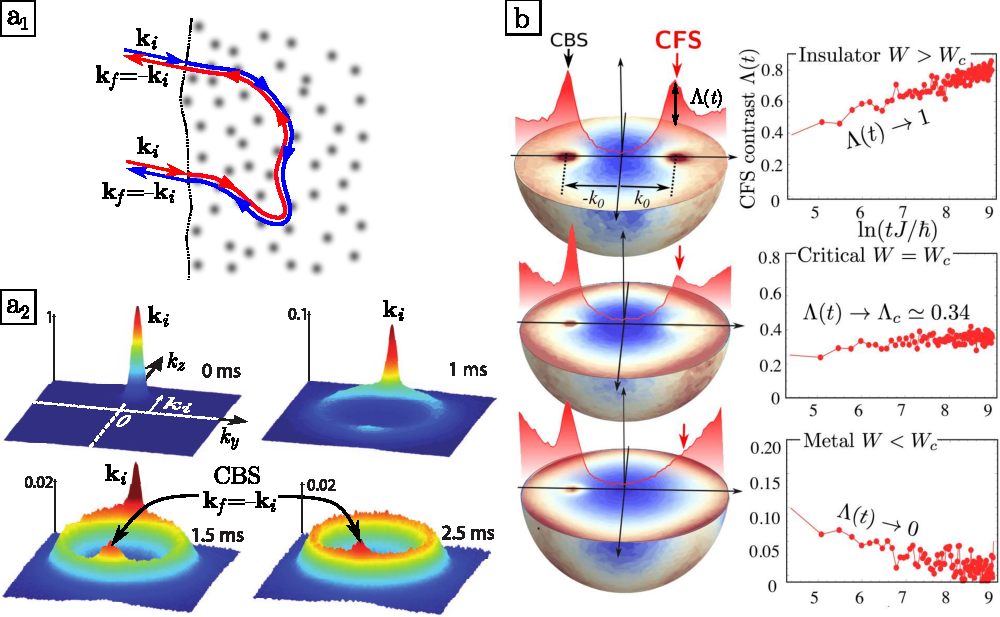
\includegraphics[width=\textwidth]{Fig/Conclusion/cbs_cfs.pdf}
\caption{\textbf{Signatures dans l'espace des vitesses.} $\mathbf{a_1}$ et $\mathbf{a_2:}$ Rétro-diffusion cohérente. Les effets de localisation faible conduisent à des interférences constructives dans la direction de rétro-diffusion, qui se manifeste sous la forme d'un pic émergeant de l'anneau de diffusion élastique dans la direction opposée à la direction initiale. \textbf{b:} Diffusion cohérente vers l'avant. Dans le régime de localisation d'Anderson, la symétrie de la distribution d'impulsion se manifeste par l'apparition d'un pic de diffusion cohérente vers l'avant aux temps longs. Il a été montré que le contraste de ce pic pouvait être considéré comme un paramètre d'ordre de la transition d'Anderson. Dans le régime diffusif, ce pic n'est pas visible et son contraste est nul. Dans le régime localisé, le contraste de ce pic tend vers $1$, par symétrie avec le CBS. Dans le régime critique, il a été montré que le contraste du CFS tend vers une valeur intermédiaire de $0.34$. }
\label{fig:cbs_cfs}
\end{figure}

Cependant, l'observation de tels effets de localisation forte sur la dynamique du CBS nécessite une résolution dans l'espace des impulsions $\Delta k_{\mathrm{res}}$ d'environ un ordre de grandeur inférieure à la résolution expérimentale actuelle. L'observation de cette signature serait un véritable tour de force expérimental.



\subsection{Diffusion cohérente vers l'avant}
Il est possible d'interpréter les états localisés comme des états liés au désordre. Pour ces états $\etat{\psi}$, l'impulsion moyenne est nulle, ce qui se traduit par
\begin{equation}
\int_{-\infty}^{+\infty}{\diff k \: k |\psi(k)|^2}=0 \text{ .}
\end{equation}
Cette condition peut se réécrire 
\begin{equation}
|\psi(k)|^2=|\psi(-k)|^2 \text{ ,}
\end{equation}
montrant que la distribution d'impulsion de ces états est symétrique. Cette symétrie est notamment décrite par l'apparition d'un pic de diffusion cohérente vers l'avant $\mathbf{k}=\mathbf{k}_{\mathrm{i}}$, découvert récemment par Karpiuk et al. \citep{karpiuk2012coherent} à l'aide de simulations numériques. Ce pic n'existant que pour des états localisés, il s'agit d'une signature dans l'espace des impulsions de la localisation d'Anderson.

L'évolution temporelle de la distribution d'impulsion dans le désordre peut alors se décomposer selon trois étapes:
\begin{itemize}
\item[\textendash] L'état initial $\etat{\mathbf{k}_{\mathrm{i}}}$ décroît avec un temps caractéristique $\taus$ et est déplété vers les autres états d'impulsion $\etat{\mathbf{k}'}$ avec $k=k_{\mathrm{i}}$. 
\item[\textendash] Après de multiples diffusions, la distribution d'impulsion devient isotrope sur une durée typique $\taub$ et le pic CBS émerge de la distribution isotrope. 
\item[\textendash] Aux temps longs, la localisation d'Anderson se manifeste dans l'espace des impulsions sous la forme du pic de diffusion cohérente vers l'avant.
\end{itemize}

Il a depuis été montré que le contraste $\Lambda$ de ce pic de diffusion cohérente vers l'avant (\emph{CFS} pour l'anglais \emph{Coherent Forward Scattering}) pouvait être utilisé comme paramètre d'ordre de la transition d'Anderson \citep{ghosh2017coherent}. En effet, il a été montré que 
\begin{equation}
\Lambda(t) \rightarrow \left\lbrace \begin{aligned}
& 0  \quad &&\text{pour } E>\Ec \text{ ,}\\
& \Lambda_{\mathrm{c}}\approx 0.34 \quad &&\text{pour } E=\Ec \text{ ,}\\
& 1 \quad &&\text{pour } E<\Ec \text{ ,}
\end{aligned}\right.
\label{eq:contraste_cfs}
\end{equation}
illustré figure \ref{fig:cbs_cfs}b.

L'observation expérimentale du pic de diffusion cohérente vers l'avant consiste un formidable défi expérimental et n'a pas encore été réalisée, excepté dans les systèmes de \emph{kicked rotor} pour lesquels l'analogue est observé dans l'espace des positions \citep{hainaut2018controlling}. Son observation en dimensions réduites nécessite une amélioration de la résolution d'impulsion $\Delta k_{\mathrm{res}}$, tandis que son observation en trois dimensions nécessite de plus une reconstruction tridimensionnelle de la fonction d'onde, avec une tomographie optique par exemple \citep{brantut2008light}. 







\section{Générer un désordre sur mesure} 
Au cours de ce manuscrit, nous nous sommes attachés à démontrer l'importance capitale de la distribution de potentiel sur les propriétés de transport. Si l'amplitude du désordre $|\VR|$ est aisément contrôlable sur notre expérience, la distribution de potentiel reste déterminée par l'équation \ref{eq:distribution_potentiel_speckle}. L'implémentation d'un modulateur spatial de lumière en remplacement du diffuseur, ou d'une matrice de micro-miroirs, permet de générer un désordre entièrement déterminé. Celui-ci permet non seulement de modifier les corrélations spatiales du désordre, mais aussi sa distribution \citep{bender2018customizing}. Une telle implémentation ouvre de nombreuses applications expérimentales, parmi lesquelles figurent un test de l'universalité de la transition d'Anderson et l'étude la transition entre localisation d'Anderson et percolation classique. 

Plus particulièrement, l'utilisation d'un modulateur spatial de lumière nous permettrait d'étudier expérimentalement la théorie de \emph{Landscape}, récemment développée par Marcel Filoche et Svitlana Mayboroda \citep{filoche2012universal}. Dans le cadre de leur théorie, les phénomènes de localisation faible et de localisation d'Anderson sont la manifestation d'un seul mécanisme universel encodé par la fonction de landscape $u$, solution de l'équation\footnote{Avec ces unités, l'équation de Schrödinger s'écrit $(-\Delta+V)\psi=E\psi$.}
\begin{equation}
(-\Delta+V)u=1 \text{ .}
\label{eq:landscape}
\end{equation}

\begin{figure}
\centering
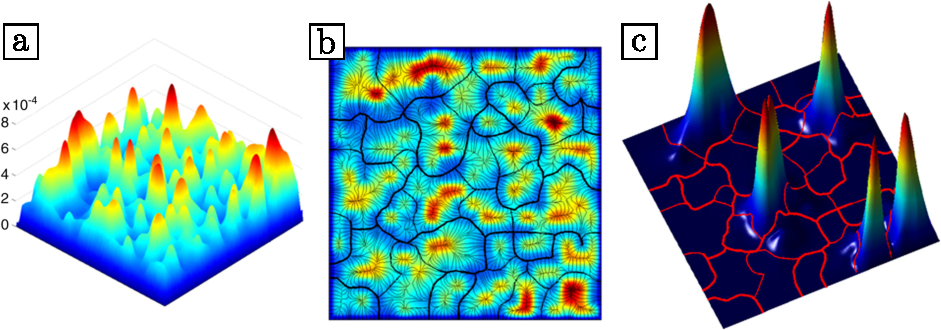
\includegraphics[width=\textwidth]{Fig/Conclusion/landscape.pdf}
\caption{\textbf{Illustration de la théorie de Landscape.} \textbf{a:} Fonction de landscape pour une réalisation du désordre calculée par l'équation \ref{eq:landscape}. \textbf{b:} Représentation de la même fonction de landscape avec son réseau de vallées pour une énergie donnée. Ce réseau de vallées délimite des sous-régions entre lesquelles la fonction d'onde est fortement atténuée. \textbf{c:} Représentation du réseau de vallées où sont superposés les premiers modes propres du système. Les vallées semblent définir les sous-régions qui supportent les modes propres associés.}
\label{fig:landscape}
\end{figure}

Les auteurs ont ainsi montré que la fonction d'onde d'un mode est fortement atténuée le long des minimas de la fonction de landscape, séparant l'espace en sous-régions délimitées par un réseau de vallées de la fonction de landscape (voir figure \ref{fig:landscape}, milieu). Finalement, les auteurs ont remarqué que ce réseau de vallées reproduisait les domaines dans lesquels les modes propres du système étaient localisés (voir figure \ref{fig:landscape}, droite). Ils interprètent ainsi le phénomène de localisation comme de la percolation dans un potentiel caché $W=1/u$.

La théorie de landscape prédit ainsi les régions de localisation et les énergies propres associées avec une précision remarquable. De plus, cette théorie ouvre la voie au \emph{problème inverse}, c'est-à-dire créer un désordre afin d'obtenir des propriétés souhaitées de localisation. Le développement récent de cette théorie suscite une très grosse activité de recherche dans le monde, dont la mise en place d'une collaboration entre les auteurs et notre équipe dans le cadre du projet \emph{SIMONS} afin de reproduire les fonctions spectrales mesurées à l'aide de la théorie de landscape.





\begin{comment}
\section{Localisation d'Anderson et interactions}

Effet des interactions: many-body localization, verre de bose...
\citep{schreiber2015observation} \citep{choi2016exploring}
\begin{figure}
\centering
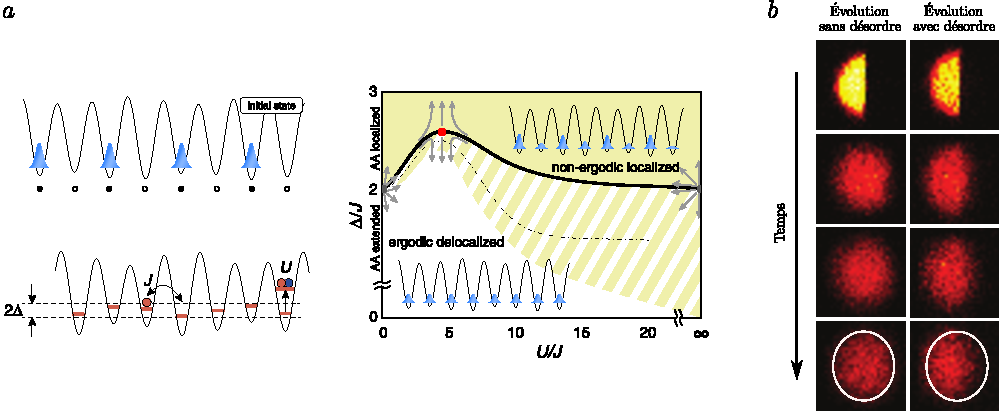
\includegraphics[width=\textwidth]{Fig/Conclusion/many_body_localisation.pdf}
\caption{\textbf{Localisation à $N$-corps.} Stuff. \\
\textbf{corriger figure de gauche.}}
\label{fig:many_body_localisation}
\end{figure}




La physique du désordre n'en est encore qu'à son balbutiement.
\end{comment}

%\makeatletter
%\def\toclevel@chapter{0}
%\makeatother